\section{Nombre: Itzpápalotl}  \label{per:itzpapalotl}
\subsection{Descripción:}
Diosa de altura media y complexión delgada. De piel blanca y ojos negros. Su larga cabellera negra va arreglada en un par de trenzas. Maquilla su cara con pintura de guerra negra. Su vestimenta es el de una guerrera, con algunas variantes del uniforme militar mexica para permitirle mayor agilidad y capacidad de vuelo.  Tiene un par de alas de mariposa hechas de obsidiana que le permiten volar y realizar ataques poderosos.    

Itzpápalotl es una diosa de actitud activa, es directa y no teme decir lo que piensa pero mide sus palabras con quienes resulten más sensibles a las palabras. Itzpápalotl toma su deber con seriedad. Es una mujer segura, con una gran fuerza de voluntad e independiente. Desafortunadamente, después de la guerra contra los Dioses del Norte, Itzpápalotl desarrollo síndrome de estrés postraumático, por lo que se le dificulta luchar; siendo Itztlacoliuhqui  el único capaz de calmarla cuando tiene episodios de crisis.
\subsection{Status:}
	\begin{itemize}
		\item Personaje no jugable.
		\item Enemigo jefe.
	\end{itemize}
\subsection{Imagen}
Ver figura \ref{fig:ItzpapalotlDiseno}
\begin{figure}
				\centering
				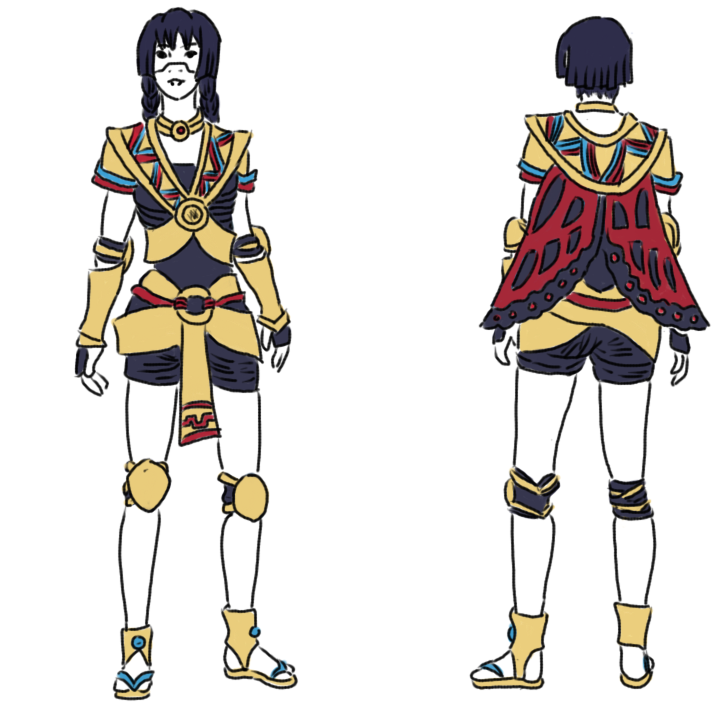
\includegraphics[height=0.3 \textheight]{Imagenes/Itzpapalotl}
				\caption{Concepto de diseño de Itzpápalotl.}
				\label{fig:ItzpapalotlDiseno}
\end{figure}
\subsection{Concepto:}
\begin{itemize}
	\item \textbf{Historia antes del juego:}
	Itzpápalotl es una de las diosas de mayor antigüedad, siendo la primera en no adoptar un rol dedicado al hogar o a la belleza, optando por ser una diosa guerrera.
	Durante los años posteriores al quinto sol, los dioses aztecas lucharon una guerra contra los dioses del norte. En esta guerra Iztpápalotl se desempeño como una capitana de gran jerarquía logrando ganar innumerables batallas. Las victorias de Itzpápalotl no hicieron otra cosa más que llenarla de orgullo, haciéndola olvidar cualquier tipo de modestia, llegando incluso a ignorar ordenes de Dioses con un rango mayor. En una de las batallas más decisivas para la guerra, Itzpápalotl se niega a pedir refuerzos provocando que todas sus tropas sean eliminadas, rodeada por sus enemigos, Izpápalotl lucha contra quinientos dioses enemigos, derrotando a una cantidad considerable de ellos pero resultando derrotada al final. Tras su derrota los dioses enemigos deciden prenderle fuego para acabar con ella. El fuego no logra matarla, pero consigue convertir su piel en cenizas. Las heridas causadas por esa batalla lograrían hacer que Itzpápalotl se retirara del campo de batalla sin la posibilidad de volver.
	
	La derrota de Iztpápalotl traería consigo un efecto en cadena en la defensa de los Dioses aztecas culminando con la perdida de la guerra. Nuevamente instaurada la paz, Itzpápalotl siente que la derrota en la guerra es producto de sus errores. Itzpápalotl le pide entonces a Tezcatlipoca que la envie al Mictlan para que pueda enmendar sus errores al fungir como una guardiana. Siendo el Mictlán el lugar donde conoceria a su futuro esposo: Itztlacoliuhqui. 
	\item \textbf{Historia durante el juego:}
	En un principio Itzpápalotl no toma muy enserio el ataque de Xólotl al Mictlán, principalmente a que las anteriores invasiones al Mictlán habían sido detenidas únicamente con el poder de Xochitónal. Su encuentro contra Xólotl y Malinalli la toma por sorpresa ya que ella confiaba en que Tepeyóllotl sería capaz de eliminar a los invasores sin ningún problema. Es precisamente su exceso de confianza lo que define su  derrota en el enfrentamiento contra Malinalli. Cuando es derrotada por Malinalli, Itzpápalotl utiliza lo último que le queda de energía para enviarle un ultimo mensaje a Itztlacoliuhqui, mostrando que por sobre su deber estaba el amor que sentía por él.
	\item \textbf{Relaciones:}
	\begin{itemize}
		\item \textbf{Itztlacoliuhqui:} Esposo de Itzpápalotl. En él Itzpápalotl encontró la calma y el lugar seguro que necesitaba. Él es quien Itzpápalotl ama más y quien ocupa su prioridad número uno (ver aparatado \ref{per:itztlacoliuhqui}).  
		\item \textbf{Tezcatlipoca:} Le permitió a Itzpápalotl integrarse a los guardianes del Mictlán luego de que perdieran la guerra contra los Dioses del norte (ver aparatado \ref{per:tezcatlipoca}).   
	\end{itemize}                     
\end{itemize}

\subsection{Encuentro:}
\begin{itemize}
	\item Su primera aparición es en la cinemática 9 (ver aparatado \ref{Cin:Cinematica09}). 
	\item Su primer y único encuentro con Malinalli es en el cuarto nivel del juego (ver aparatado \ref{Nivel:Niv04}).
\end{itemize}
\subsection{Habilidades:}
\begin{itemize}
	\item Circulo de fuego (ver aparatado \ref{hab.CirFue}).
	\item Embestida aerea (ver aparatado \ref{hab.EmbesAer}).
	\item Invisibilidad (ver aparatado \ref{hab.Invis}).
\end{itemize}
\subsection{Armas:})
Matlalpapalotl (ver aparatado \ref{Arma:LanzaItzpapalotl}).
\subsection{Ítems:}
Sin ítems.

\subsection{Bloques de animación}
 	\begin{itemize}
		\item Animación disparar fuego.
		\item Animación embestida.
		\item Animación caminar.
		\item Animación desvanecerse.
		\item Animación aparecer.
    \end{itemize}